\section{Introduction}

These courses are supposed to give you an overview of the kind of statistical issues you're likely to face during your PhD, when analysing experimental data. Often the kind of issues we high energy physicists deal with are not the same as for statisticians dealing with survey questionnaires, financial traders dealing with index price fluctuations or epidemiologists dealing with viral outbreaks. However, some of the fundamental concepts of course are the same (even if in practise it leads to very different levels of rigour). 

These lectures are therefore not meant to be a complete course in statistics theory, but rather a practical course focused on the most common statistical methods used in HEP. I'm basing a lot of this material on an excellent book by Frederick James, \emph{``Statistical Methods in Experimental Physics: 2nd Edition,''} (see Figure~\ref{fig:james} below). I strongly recommend this book for further reading on statistics for high energy particle physics. 

\begin{figure}[hbt!]
    \centering
    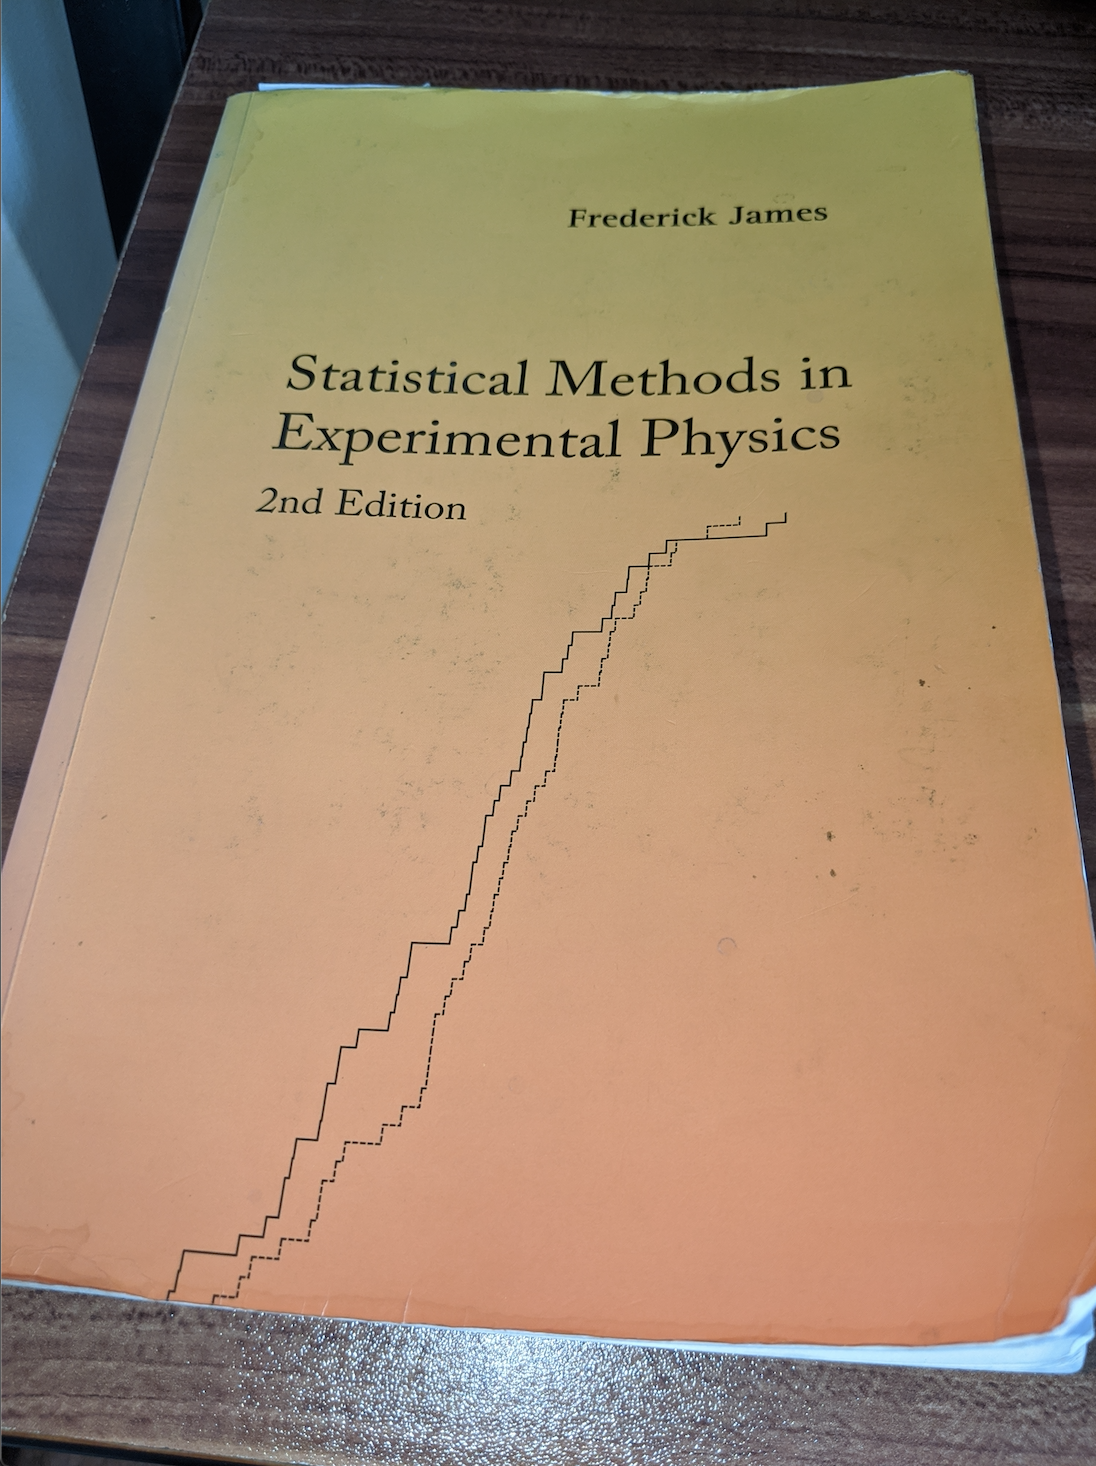
\includegraphics[width=0.5\textwidth]{figures/intro/james.png}
    \caption{My beaten up copy of James, coffee stains and all.}
    \label{fig:james}
\end{figure}

While the theory behind the statistical methods we'll cover is vital to understand what we do and why we do it, the practicality of using those methods is equally important for a successful PhD in HEP. These lectures will include some element of programming to give you an idea as to how to code up the methods for your own research. Since every collaboration/experiment will have their own fitting/statistics software, and since there are many industry standards out there, I'll try to simple code without using too many fancy packages. For the problems, feel free to use whatever you like concerning languages/packages to get the solutions. I'll be interested in seeing what you can come up with. A few examples of good languages for programming statistics are \textsf{R, python, ROOT (C++ based), Mathematica...} and of course there are plenty of tools for complicated statistical routines and workflows such as \textsf{PyTorch, tensorflow, Stan, Minuit (iMinuit), RooFit/RooStats, pyHF, HistFitter/HistFactory, Combine ...}. 
Whenever there is a snippet of code to explain something, you'll see a code box like the following. 

\begin{lstlisting}[style = Python]
# basic Python codeblock
nothing = [print("hello") for i in range(10)]
# or the for loop version
for i in range(10): 
  print("hello")
\end{lstlisting}

I'll tend to use \textsf{python 3}, but you should not let that discourage you from using another language if you prefer. We care about the statistics in the end. All of the code examples in these lectures can be found in full on \textsf{GutHub} at  \url{https://github.com/nucleosynthesis/PGStatistics}. You can follow along by either checking out the repository and running the notebooks (in the  \textsf{notebooks} folder) or launching a python interpreter to run in your browser by either clicking the button that looks like this: 
\includegraphics[height=1.2\fontcharht\font`\B]{figures/binder.png}, or by clicking \href{https://mybinder.org/v2/gh/nucleosynthesis/PGStatistics/main?urlpath=lab}{this link}. 

By the end of this course, you should have an idea of what a particle physicist means by an ``limit'', a ``significant result'' and what is really meant by a ``measured value of  $X+\pm \sigma_{X}$''. Furthermore, you should be able to calculate such things yourself using some simple programming tools.  

